\documentclass[aspectratio=169]{beamer}


\usepackage[brazil]{babel}
\usepackage[utf8]{inputenc}
\usepackage{algorithm, algpseudocode}
\usepackage{graphicx}
\usepackage{subfig}
\usepackage{multicol}
\usepackage{verbatim}
\usepackage[absolute]{textpos}
\usepackage{todonotes}\presetkeys{todonotes}{inline}{}
\usepackage{minted}
\makeatletter
\renewcommand{\ALG@beginalgorithmic}{\small}
\makeatother

\usetheme[progressbar=foot]{metropolis}

\title{Arquitetura de Computadores}
\subtitle{Dispositivos Lógico Programáveis (\textit{Hardware} Reconfigurável) \\ Arranjo de Portas Programável em Campo - FPGA}
\date{Última Atualização: \today}
\author{Rodolfo Labiapari Mansur Guimarães}

\institute{
	\textit{rodolfolabiapari@gmail.com} \\
	Lattes: \url{http://goo.gl/MZv4Dc} \\
	Departamento de Computação -- Universidade Federal de Ouro Preto \\
		Ouro Preto - MG -- Brasil }



\begin{document}
\maketitle

\usebackgroundtemplate{
\includegraphics[trim=0 245cm 0 0, width=0.05\textwidth]{img/ufop.jpg}}


\begin{frame}{Sobre esta Aula}
		\pause
		\centering
		\Large
		``\textit{Não existe pergunta idiota, existe idiota que não pergunta}''.
\end{frame}

	\begin{frame}{Sobre Mim}
		\begin{itemize}
			\setlength\itemsep{1.3em}
			\item \textbf{Formação:} Instituto Federa de Educação, Ciência e Tecnologia de Minas Gerais (IFMG) - Campus Formiga.
			\item \textbf{Pesquisas Aplicadas:}
			\begin{itemize}
				\setlength\itemsep{0.7em}
				\item Projeto e Desenvolvimento de um Carro Robô controlado por \textit{Smartphone}, Utilizando a Plataforma Amarino (Google Android e Arduino);
				\item Projeto e Desenvolvimento de um \textit{Hardware} Reconfigurável de Criptografia para a Transmissão Segura de Dados.
			\end{itemize}
			
			\item \textbf{Trabalho de Conclusão de Curso:}
			\begin{itemize}
				\item Desenvolvimento de um \textit{Device Driver} para Comunicação com um \textit{Hardware} Reconfigurável.
			\end{itemize}
			
			\item \textbf{Lattes:} \url{http://goo.gl/MZv4Dc}.
		\end{itemize}
	\end{frame}

\section{Matemática Discreta - \newline Lógica Proposicional e Eletrônica Digital}
	\begin{frame}{Lógica e Eletrônica - Tabelas Verdades}
		\begin{itemize}
			\item Chamamos \textbf{tabela verdade} de uma função booleana a tabela que apresenta \textbf{os valores da função} $ y = f(A, B) $ para \textbf{todas as combinações possíveis} dos valores das variáveis.
		\end{itemize}
		
		\begin{multicols}{2}
			\begin{figure}[h]
				\centering
				\caption{Exemplo de tabela verdade com 2 entradas}
				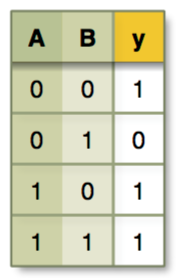
\includegraphics[height=0.35\textheight]{img/ed/ed-tabela_verdade.png}
				\\
				{\footnotesize \textbf{Fonte:} Disponível em: \url{http://eletro.g12.br/arquivos/materiais/eletronica4.pdf}.}
				\label{fig:ed-tabela_verdade}
			\end{figure}
			\columnbreak
			\begin{itemize}
				\item Tabela é \textbf{uma} de várias formas de representação de funções lógicas.
			\end{itemize}
		\end{multicols}
	\end{frame}
	
	\begin{frame}{Lógica e Eletrônica - Tabelas Verdades}
			\begin{figure}[h]
				\centering
				\caption{Exemplo de tabela verdade com 3 entradas}
				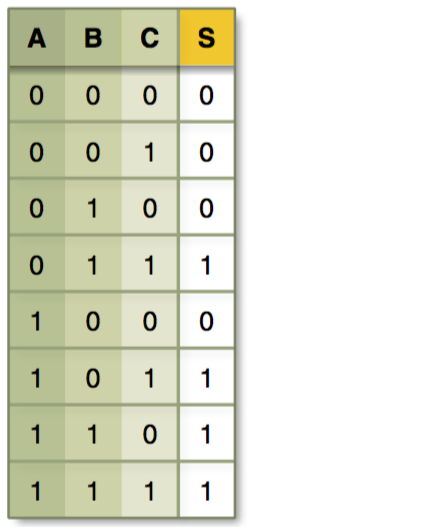
\includegraphics[height=0.7\textheight]{img/ed/ed-tabela_circuito1.png}
				\\
				{\footnotesize \textbf{Fonte:} Disponível em: \url{http://eletro.g12.br/arquivos/materiais/eletronica4.pdf}.}
				\label{fig:ed-tabela_circuito1}
			\end{figure}
	\end{frame}
	
	\begin{frame}{Lógica e Eletrônica - Tabelas Verdades}
			\begin{figure}[h]
				\centering
				\caption{Exemplo de tabela verdade com 3 entradas }
				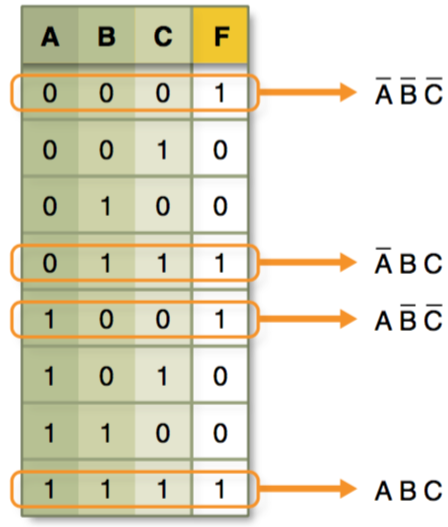
\includegraphics[height=0.7\textheight]{img/ed/ed-tabela_circuito2.png}
				\\
				{\footnotesize \textbf{Fonte:} Disponível em: \url{http://eletro.g12.br/arquivos/materiais/eletronica4.pdf}.}
				\label{fig:ed-tabela_circuito2}
			\end{figure}
	\end{frame}

	\begin{frame}{Lógica e Eletrônica - Portas Lógicas}
		\begin{itemize}
			\setlength\itemsep{1.5em}
			\item Portas lógicas são \textbf{circuitos eletrônicos básicos} que possuem uma ou mais entradas e uma única saída.
			
			\item Nas entradas e na saída, podemos associar valores booleanos. 
			
				\bigskip
			
			\item Em eletrônica digital atribuímos valores de tensão 
			\begin{itemize}
				\item Associamos ao $ 5 $ V o estado ``$ 1 $'' e ao $ 0 $ V, o estado ``$ 0 $''.
			\end{itemize}
		\end{itemize}
	\end{frame}
	
	
	\begin{frame}{Lógica e Eletrônica - Portas Lógicas - Porta NOT}
		\begin{figure}[h]
			\centering
			\caption{Representação da Porta Lógica NOT}
			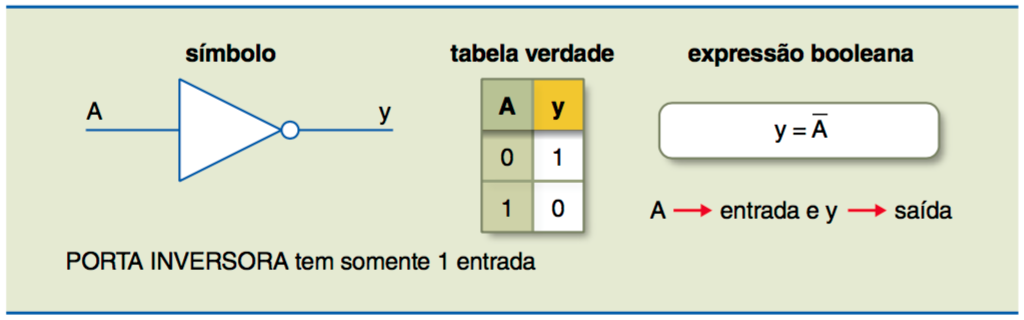
\includegraphics[height=0.55\textheight]{img/ed/ed-porta_not.png}
			\\
			{\footnotesize \textbf{Fonte:} Disponível em: \url{http://eletro.g12.br/arquivos/materiais/eletronica4.pdf}.}
			\label{fig:ed-porta_NOT}
		\end{figure}
	\end{frame}
	
	\begin{frame}{Lógica e Eletrônica - Portas Lógicas - Porta AND}
		\begin{figure}[h]
			\centering
			\caption{Representação da Porta Lógica AND}
			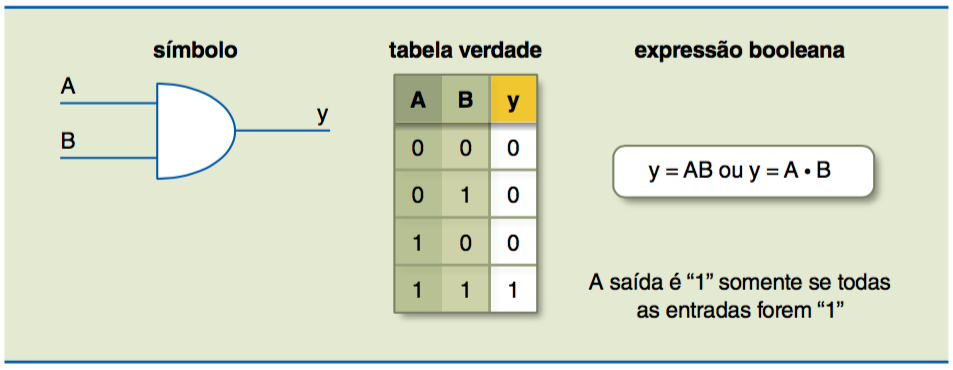
\includegraphics[height=0.66\textheight]{img/ed/ed-porta_and.png}
			\\
			{\footnotesize \textbf{Fonte:} Disponível em: \url{http://eletro.g12.br/arquivos/materiais/eletronica4.pdf}.}
			\label{fig:ed-porta_AND}
		\end{figure}
	\end{frame}
	
	\begin{frame}{Lógica e Eletrônica - Portas Lógicas - Porta NAND}
		\begin{figure}[h]
			\centering
			\caption{Representação da Porta Lógica NAND}
			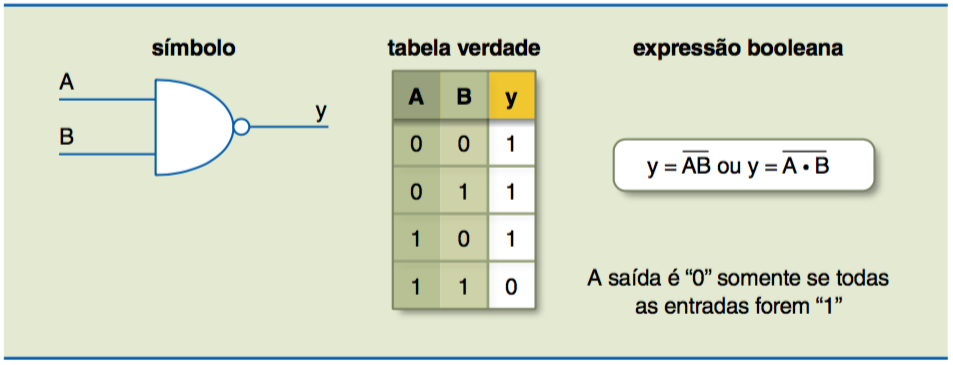
\includegraphics[height=0.66\textheight]{img/ed/ed-porta_nand.png}
			\\
			{\footnotesize \textbf{Fonte:} Disponível em: \url{http://eletro.g12.br/arquivos/materiais/eletronica4.pdf}.}
			\label{fig:ed-porta_NAND}
		\end{figure}
	\end{frame}
	
	\begin{frame}{Lógica e Eletrônica - Portas Lógicas - Porta OR}
		\begin{figure}[h]
			\centering
			\caption{Representação da Porta Lógica OR}
			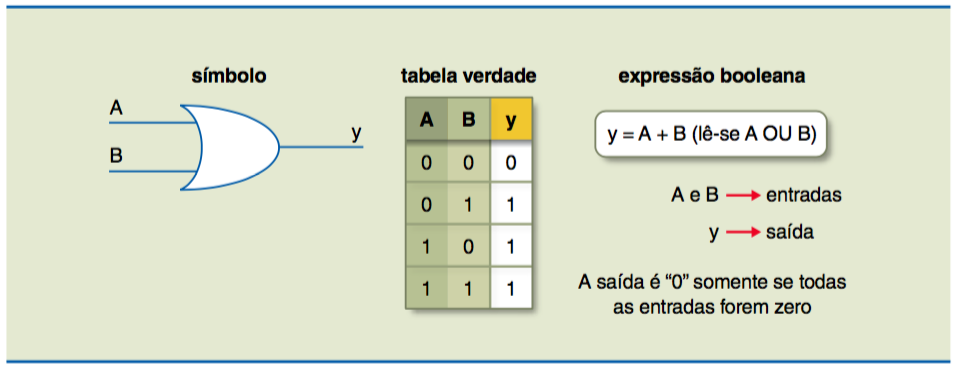
\includegraphics[height=0.66\textheight]{img/ed/ed-porta_or.png}
			\\
			{\footnotesize \textbf{Fonte:} Disponível em: \url{http://eletro.g12.br/arquivos/materiais/eletronica4.pdf}.}
			\label{fig:ed-porta_OR}
		\end{figure}
	\end{frame}
	
	\begin{frame}{Lógica e Eletrônica - Portas Lógicas - Porta NOR}
		\begin{figure}[h]
			\centering
			\caption{Representação da Porta Lógica NOR}
			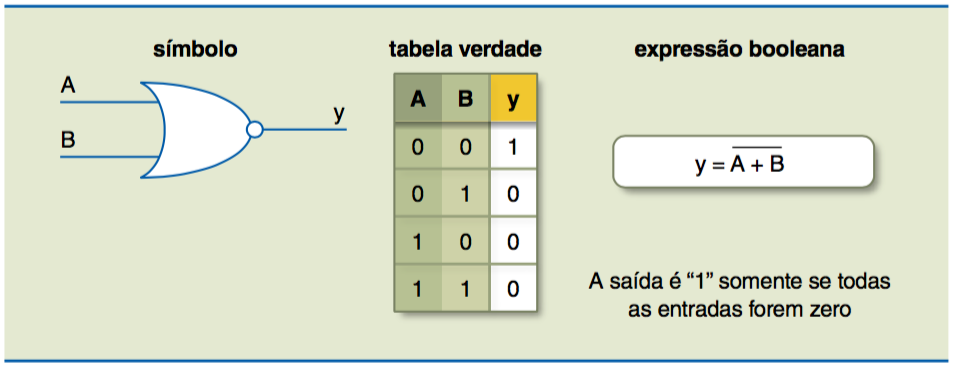
\includegraphics[height=0.66\textheight]{img/ed/ed-porta_nor.png}
			\\
			{\footnotesize \textbf{Fonte:} Disponível em: \url{http://eletro.g12.br/arquivos/materiais/eletronica4.pdf}.}
			\label{fig:ed-porta_NOR}
		\end{figure}
	\end{frame}
	
	\begin{frame}{Lógica e Eletrônica - Portas Lógicas - Porta XOR}
		\begin{figure}[h]
			\centering
			\caption{Representação da Porta Lógica XOR}
			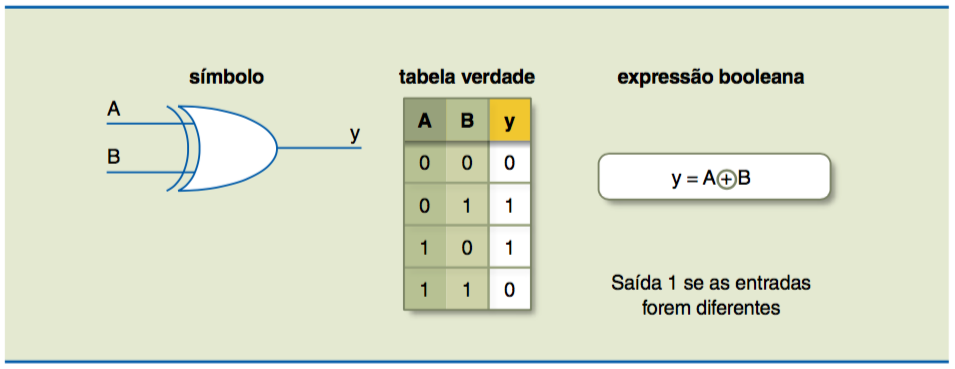
\includegraphics[height=0.66\textheight]{img/ed/ed-porta_xor.png}
			\\
			{\footnotesize \textbf{Fonte:} Disponível em: \url{http://eletro.g12.br/arquivos/materiais/eletronica4.pdf}.}
			\label{fig:ed-porta_XOR}
		\end{figure}
	\end{frame}
	
	\begin{frame}{Lógica e Eletrônica - Portas Lógicas - Porta XNOR}
		\begin{figure}[h]
			\centering
			\caption{Representação da Porta Lógica XNOR}
			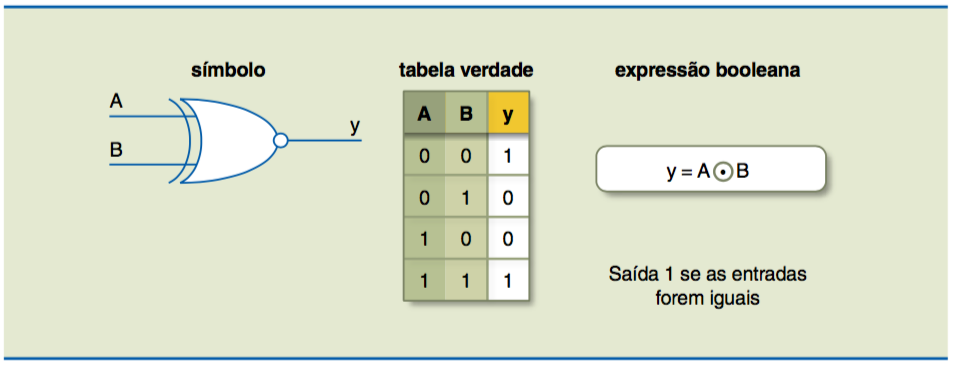
\includegraphics[height=0.66\textheight]{img/ed/ed-porta_xnor.png}
			\\
			{\footnotesize \textbf{Fonte:} Disponível em: \url{http://eletro.g12.br/arquivos/materiais/eletronica4.pdf}.}
			\label{fig:ed-porta_XNOR}
		\end{figure}
	\end{frame}
	
	\begin{frame}{Lógica e Eletrônica - Circuito Digital}
		\begin{figure}[h]
			\centering
			\caption{Representação de um circuito simples}
			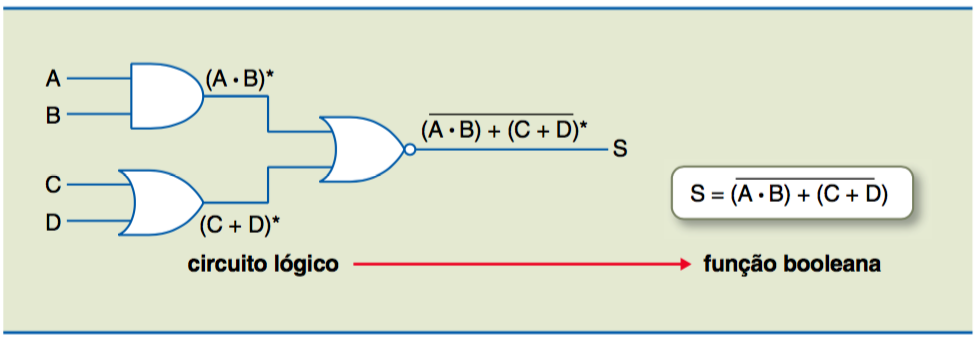
\includegraphics[height=0.6\textheight]{img/ed/ed-circuito.png}
			\\
			{\footnotesize \textbf{Fonte:} Disponível em: \url{http://eletro.g12.br/arquivos/materiais/eletronica4.pdf}.}
			\label{fig:ed-circuito}
		\end{figure}
	\end{frame}
\begin{comment}

	\begin{frame}{Lógica e Eletrônica - Circuito Digital - Circuito Integrado 74147}
		\begin{multicols}{2}
			\begin{figure}[h]
				\centering
				\caption{Circuito Integrado 74147 - codificador com prioridade decimal-BCD}
				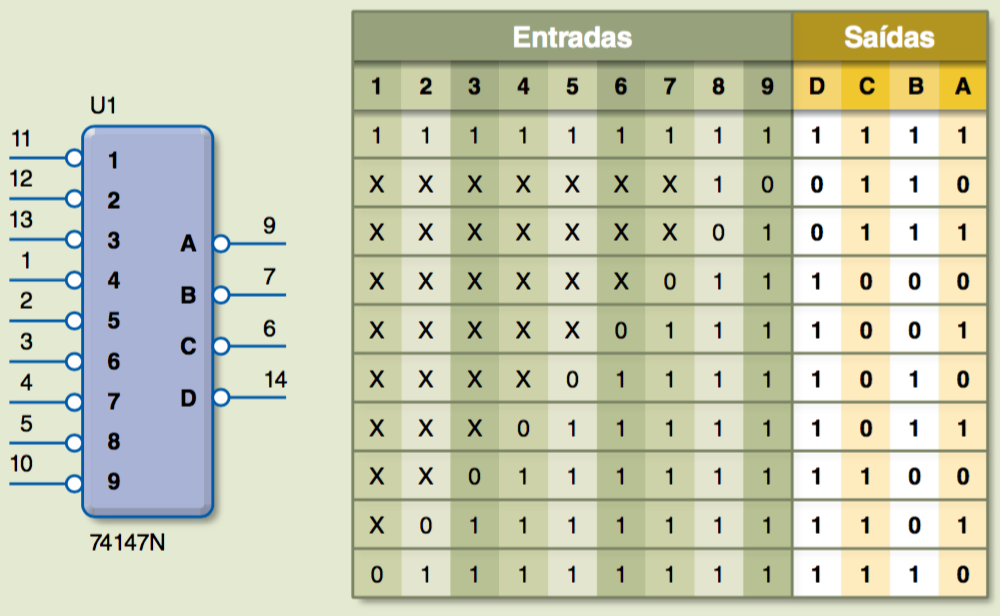
\includegraphics[height=0.6\textheight]{img/ed/ed-74147-tabela.png}
				\\
				{\footnotesize \textbf{Fonte:} Disponível em: \url{http://eletro.g12.br/arquivos/materiais/eletronica4.pdf}.}
				\label{fig:ed-74147-tabela}
			\end{figure}
			\columnbreak
			\pause
			\begin{figure}[h]
				\centering
				%\caption{Exemplo de tabela verdade com 2 entradas}
				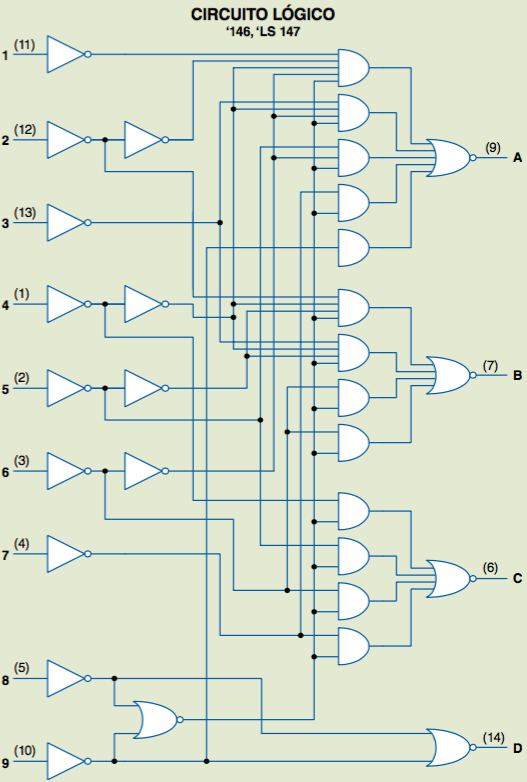
\includegraphics[height=0.93\textheight]{img/ed/ed-74147-circuito.png}
				\label{fig:ed-74147-circuito}
			\end{figure}
		\end{multicols}
	\end{frame}
	
\end{comment}
	
	\begin{frame}{Lógica e Eletrônica - Introdução ao Assunto}
		\begin{block}{Questão: Porque falar sobre Portas Lógicas se o assunto da aula é \textit{Hardware} Reconfigurável?}
			\begin{itemize}
				\item Circuitos comprado hoje, como um processador, não permitem que sejam alterados.
				
				\item E se 
			\end{itemize}
		\end{block}
	\end{frame}


\section{Dispositivos Lógico Programáveis}
	\begin{frame}{Dispositivos Lógico Programáveis}
		\begin{figure}[H]
			\centering
			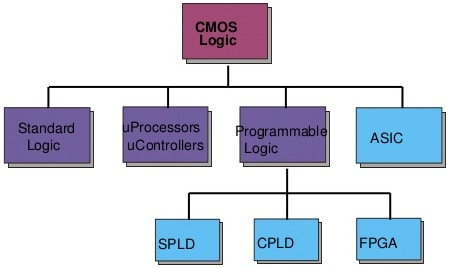
\includegraphics[width=0.9\textwidth]{img/intro/arvore.jpg}
			\caption{ASIC vs. PLD.}
		\end{figure}
	\end{frame}
	
	\begin{frame}{Dispositivos Lógico Programáveis}
		\begin{figure}[H]
			\centering
			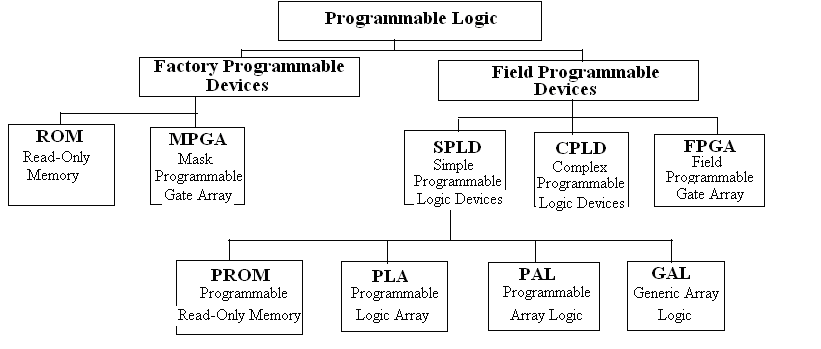
\includegraphics[width=1.08\textwidth]{img/intro/arvore-pld.png}
			\caption{\textit{Programmable Logic Device}.}
		\end{figure}
	\end{frame}
	
	\begin{frame}{Dispositivos Lógico Programáveis}
		\begin{itemize}
			\setlength\itemsep{1em}
			
			\item Tocci \cite{Tocci2003} cita que os dispositivos lógicos programáveis (PLD\footnote{do inglês \textit{Programmable Logic Device}.}) são as ``\textit{maravilhas de flexibilidade de projeto}''.
			
			\item Ao contrário de uma porta lógica, que tem uma função fixa, um PLD tem uma função indefinida após a sua fabricação. 
			
			\item Para utilizá-lo em um circuito, deve-se \textbf{programá-lo previamente}.
			
			\item A lógica programável proporciona ao projetista:
			\begin{itemize}
				\setlength\itemsep{0.3em}
				\item A possibilidade de se \textbf{adequar aos vários níveis de projetos} sendo estes:
				\begin{itemize}
					\item Para desenvolvimento de protótipos ou mesmo circuitos finais.
				\end{itemize}
				
				\item \textbf{Fácil alteração} do projeto a \textbf{qualquer momento};
				
				\item Programação por meio de Álgebra Boole, Mapa de Karnaugh, e Linguagens de Descrição de \textit{Hardware}.
			\end{itemize}
		\end{itemize}
	\end{frame}
	
	\begin{frame}{Dispositivos Lógico Programáveis}
		\begin{figure}[H]
			\centering
			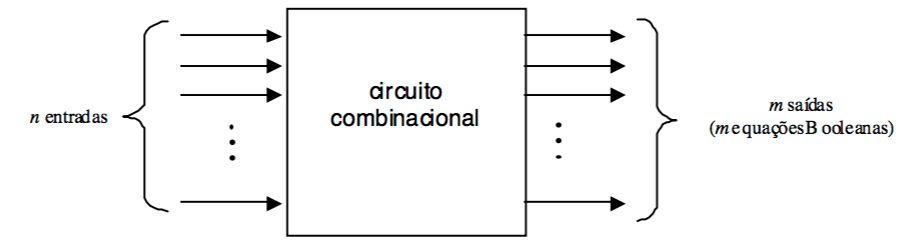
\includegraphics[width=1\textwidth]{img/fpga/geral1.png}
			\caption{Exemplo de um circuito combinacional.}
		\end{figure}
	\end{frame}
	
	\begin{frame}{Dispositivos Lógico Programáveis - FPGA}
		\begin{itemize}			
			\setlength\itemsep{0.6em}
			
			\item Em meados dos anos 80, a empresa \textbf{Xilinx} e Gerald Estrin anuncia uma nova arquitetura.
			
			\begin{itemize}
				\item Isso foi um \textbf{choque} na época pois cria-se então um \textbf{novo paradigma de projetos de circuitos integrados};
				
				\item Entre vários tipos de PLD existe um tipo que é baseado na tecnologia \textit{gate array} e é chamado de FPGA\footnote{Do inglês \textit{Field-Programmable Gate Array}, Arranjo de Portas Programável em Campo.}.
			\end{itemize}
			
			
			\item O FPGA usa uma rede de portas lógicas cuja programação é feita pelo \textbf{projetista e não pelo fabricante}. 
			\begin{itemize}
				\item Sendo reprogramados, o usuário pode utilizá-lo num projeto e logo em seguida reprogramá-lo para que execute outro projeto.
			\end{itemize}
			
			\item Deixando mais claro, o termo ``\textbf{campo}'' na nomenclatura é apenas um termo da engenharia utilizado para indicar o \textbf{mundo de fora da fábrica}.
		\end{itemize}
	\end{frame}
	
	\begin{frame}{Dispositivos Lógico Programáveis - FPGA}
		\begin{itemize}
			\setlength\itemsep{1.1em}
			
			\item Excelentes para \textbf{desenvolver um protótipo de circuito integrado} a fim da realização de testes \textbf{antes da fabricação em massa} \cite{Skliarova2003} e \textbf{ensino}.
			
			\item Seu custo em relação ao ASIC\footnote{Do inglês \textit{Application Specific Integrated Circuits}.} é menor;
			
			\item Seu tempo total gasto desde a especificação do projeto até sua sintetização também é menor
			\begin{itemize}
				\setlength\itemsep{0.5em}
				
				\item ASICs são produzidos geralmente em \textbf{larga} escala
				\begin{itemize}
					\item O custo de fabricação de 1 circuito é caro;
					\item O custo de fabricação em massa também é caro.
				\end{itemize}
				
				\item Qualquer erro no ASIC, deve-se reiniciar todo o processo de desenvolvimento
				\begin{itemize}
					\item Sendo que no FPGA isso levaria talvez algumas horas/minutos e custo zero.
				\end{itemize}
				
				\item Circuitos feitos manualmente...
			\end{itemize}
			
		\end{itemize}
	\end{frame}
	
	
	\begin{frame}{Dispositivos Lógico Programáveis - FPGA - Projetando um Circuito}
		\begin{enumerate}
			\setlength\itemsep{1em}
			\item \textbf{Descrição em Alto Nível};
			\item \textbf{Simulação Lógica};
			\pause
			\item Síntese e Mapeamento;
			\item Distribuição dos Blocos Lógicos e Roteamento dos Sinais;
			\item Análise Temporal e Simulação;
			\pause
			\item Configuração de Dispositivos de Lógica Programável;
			\pause
			\item \textbf{Teste de Avaliação}.
		\end{enumerate}
	\end{frame}
	

\section{FPGA - Hardware}
	\begin{frame}{FPGA - Hardware - Visão Geral}
		\begin{itemize}
			\setlength\itemsep{1.5em}
			\item Nos FPGAs, sua configuração é totalmente \textbf{volátil}
			\begin{itemize}
				\setlength\itemsep{1em}
				\item O projeto deve ser \textbf{recarregada} sempre que é \textbf{ligada};
				\item Para isso, a configuração é normalmente guardada numa memória não volátil como a EEPROM.
			\end{itemize}
			
			\item Internamente:
			\begin{itemize}
				\setlength\itemsep{1em}
				\item Consiste num \textbf{arranjo de blocos lógicos} e \textbf{canais de roteamento}.
			
				\item Significa que é capaz de alterar seus caminhos de dados/fluxos \textbf{habilitando/desabilitando módulos} \cite{moreira2008}.
			\end{itemize}
		\end{itemize}
	\end{frame}
	
	
	\begin{frame}{FPGA - Hardware - Visão Geral}
		\begin{figure}[h]
			\centering
			\caption{``FPGA é um \textit{quadro negro} que pode ser \textit{desenhado} qualquer circuito digital''.}
			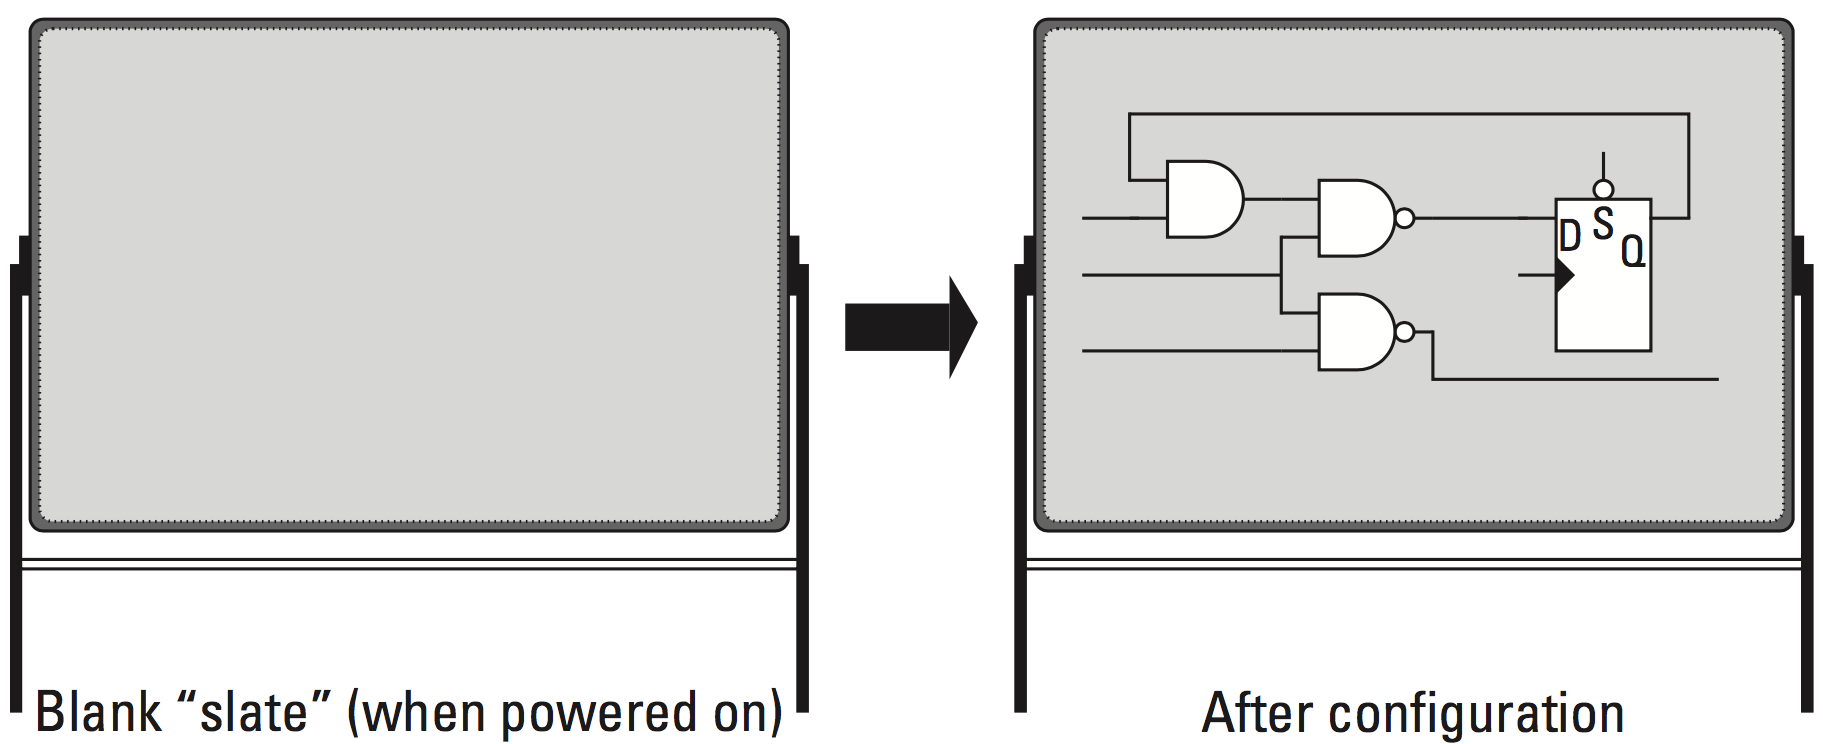
\includegraphics[height=0.7\textheight]{img/fpga/quadro.png}
			\label{fig:quadro}
		\end{figure}
	\end{frame}
	
	\begin{frame}{FPGA - Hardware - Roteamento de Blocos}
		\begin{multicols}{2}
			\begin{figure}[h]
				\centering
				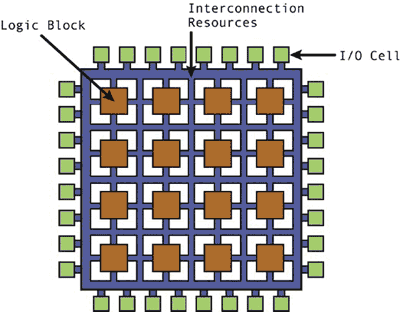
\includegraphics[width=0.55\textwidth]{img/fpga/exempo-simples.png}
				\caption{Exemplo de roteamento interno.}
				\label{fig:exempo-simples}
			\end{figure}
			\columnbreak
			Três módulos:
			\begin{itemize}
				\setlength\itemsep{1.8em}
				\item Blocos de Entrada e Saída;
				
				\item Blocos Lógicos Configuráveis;
				
				\item Chaves de Interconexão.
			\end{itemize}
		\end{multicols}
	\end{frame}
	
	\begin{frame}{FPGA - Hardware - Roteamento de Blocos}
		\begin{multicols}{2}
			\begin{figure}[h]
				\centering
				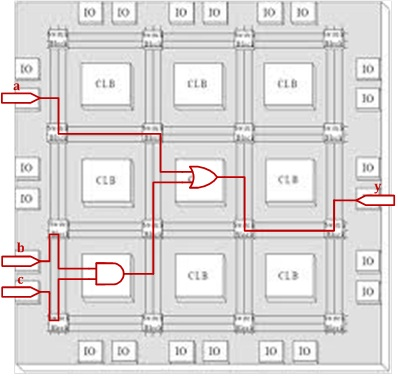
\includegraphics[width=0.45\textwidth]{img/fpga/exemplo.jpg}
				\caption{Outro exemplo de roteamento interno no FPGA.}
				\label{fig:exemplo}
			\end{figure}
			\columnbreak
			Três módulos:
			\begin{itemize}
				\setlength\itemsep{1.8em}
				\item Blocos de Entrada e Saída;
				
				\item Blocos Lógicos Configuráveis;
				
				\item Chaves de Interconexão.
			\end{itemize}
		\end{multicols}
	\end{frame}
	
	\begin{frame}{FPGA - Hardware - Roteamento de Blocos}
		\begin{figure}[H]
			\centering
			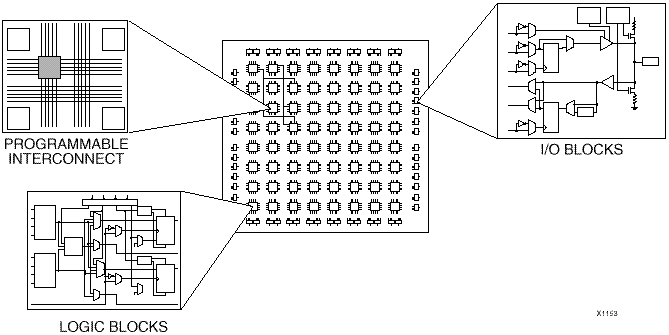
\includegraphics[width=0.97\textwidth]{img/fpga/demonstracao_2.png}
			\caption{Demonstração mais complexa de síntese.}
		\end{figure}
	\end{frame}
	
	
	\begin{frame}{FPGA - Hardware - Roteamento de Blocos}
		\begin{multicols}{2}
			\begin{figure}[h]
				\centering
				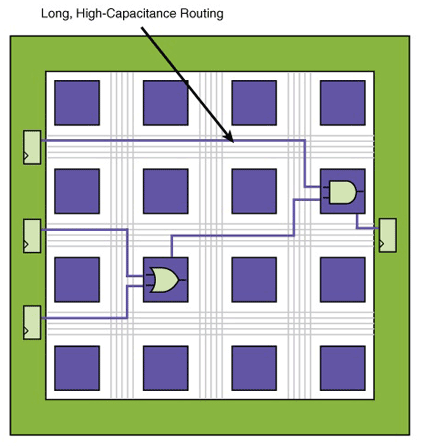
\includegraphics[width=0.40\textwidth]{img/fpga/exemploInicial.png}
				\caption{Exemplo de roteamento interno.}
				\label{fig:exemploInicial}
			\end{figure}
			\columnbreak
			\begin{itemize}
				\setlength\itemsep{1em}
				\item O FPGA \textbf{não possui funções lógicas} como AND, OR... 
				\begin{itemize}
					\item Seu arranjo de células reconfiguráveis permite a \textbf{implementação} dessas portas/tabelas.
				\end{itemize}
				
				\item Distribuições lógicas ruins e encaminhamentos mal feitos geram atrasos de processamento
				\begin{itemize}
					\setlength\itemsep{0.3em}
					\item Estudar qual a melhor maneira projetar cada circuito;
					
					\item A implementação afeta diretamente seu seu design e por fim, no desempenho.
				\end{itemize}
				
			\end{itemize}
		\end{multicols}
	\end{frame}
	
	\begin{frame}%{FPGA - Hardware - Roteamento de Blocos}
		\begin{figure}[h]
			\centering
			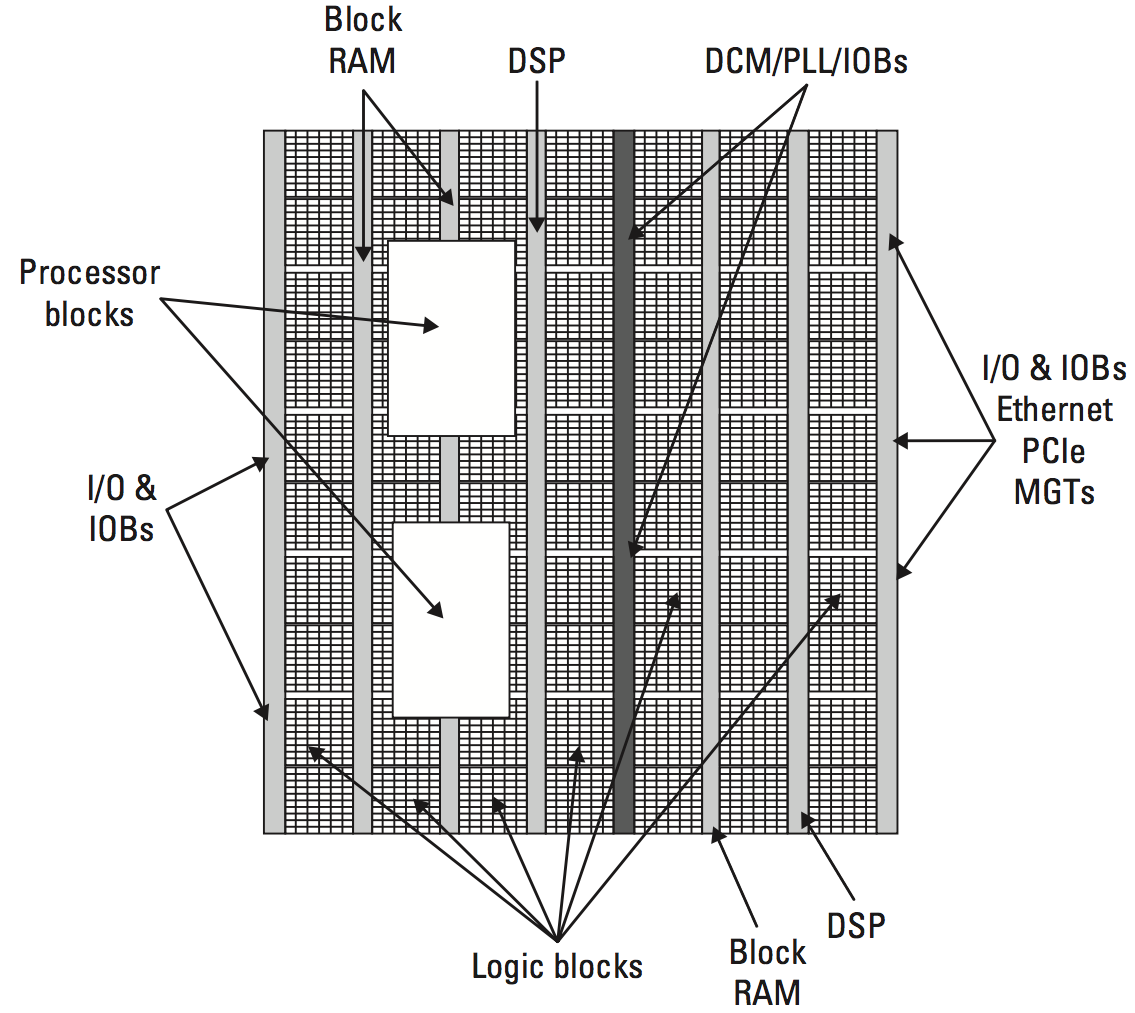
\includegraphics[height=1\textheight]{img/fpga/abstracao.png}
			\caption{Abstração de um FPGA.}
			\label{fig:abstracao}
		\end{figure}
	\end{frame}
	
	\begin{frame}%{FPGA - Hardware - Roteamento de Blocos}
		\begin{figure}[h]
			\centering
			\includegraphics[width=0.56\textwidth]{img/fpga/exemploFinal.png}
			\caption{Exemplo de roteamento interno complexo no FPGA.}
			\label{fig:exemploFinal}
		\end{figure}
	\end{frame}
	
	\begin{frame}{FPGA - Hardware - Placa}
		\begin{figure}[p]
			\centering
			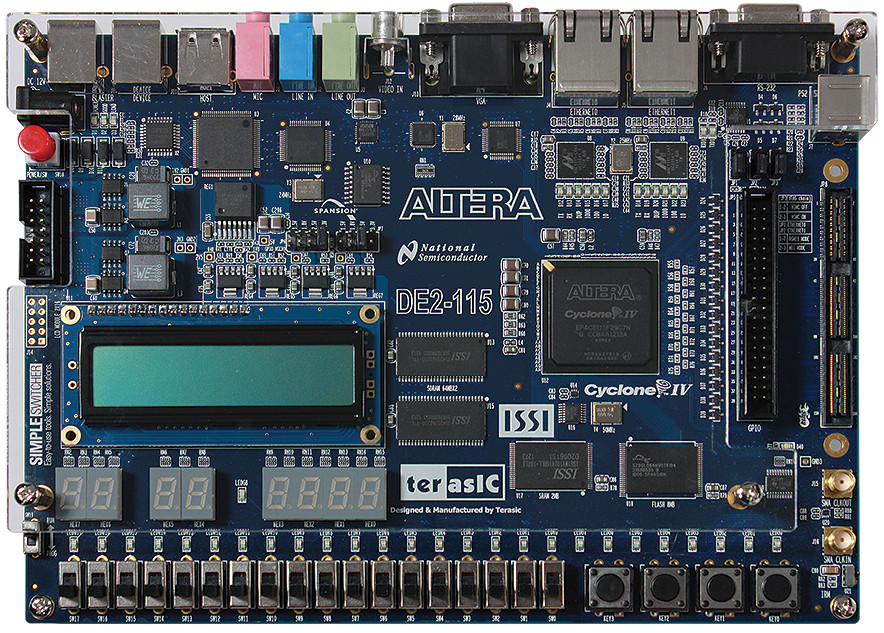
\includegraphics[width=0.68\textwidth]{img/fpga/terasic_placa.jpg}
			\caption{FPGA de Desenvolvimento Altera DE2-115.}
			\label{fig:terasic_placa}
		\end{figure}
	\end{frame}
	
	\begin{frame}%{FPGA - Hardware - Placa}
		\begin{figure}[p]
			\centering
			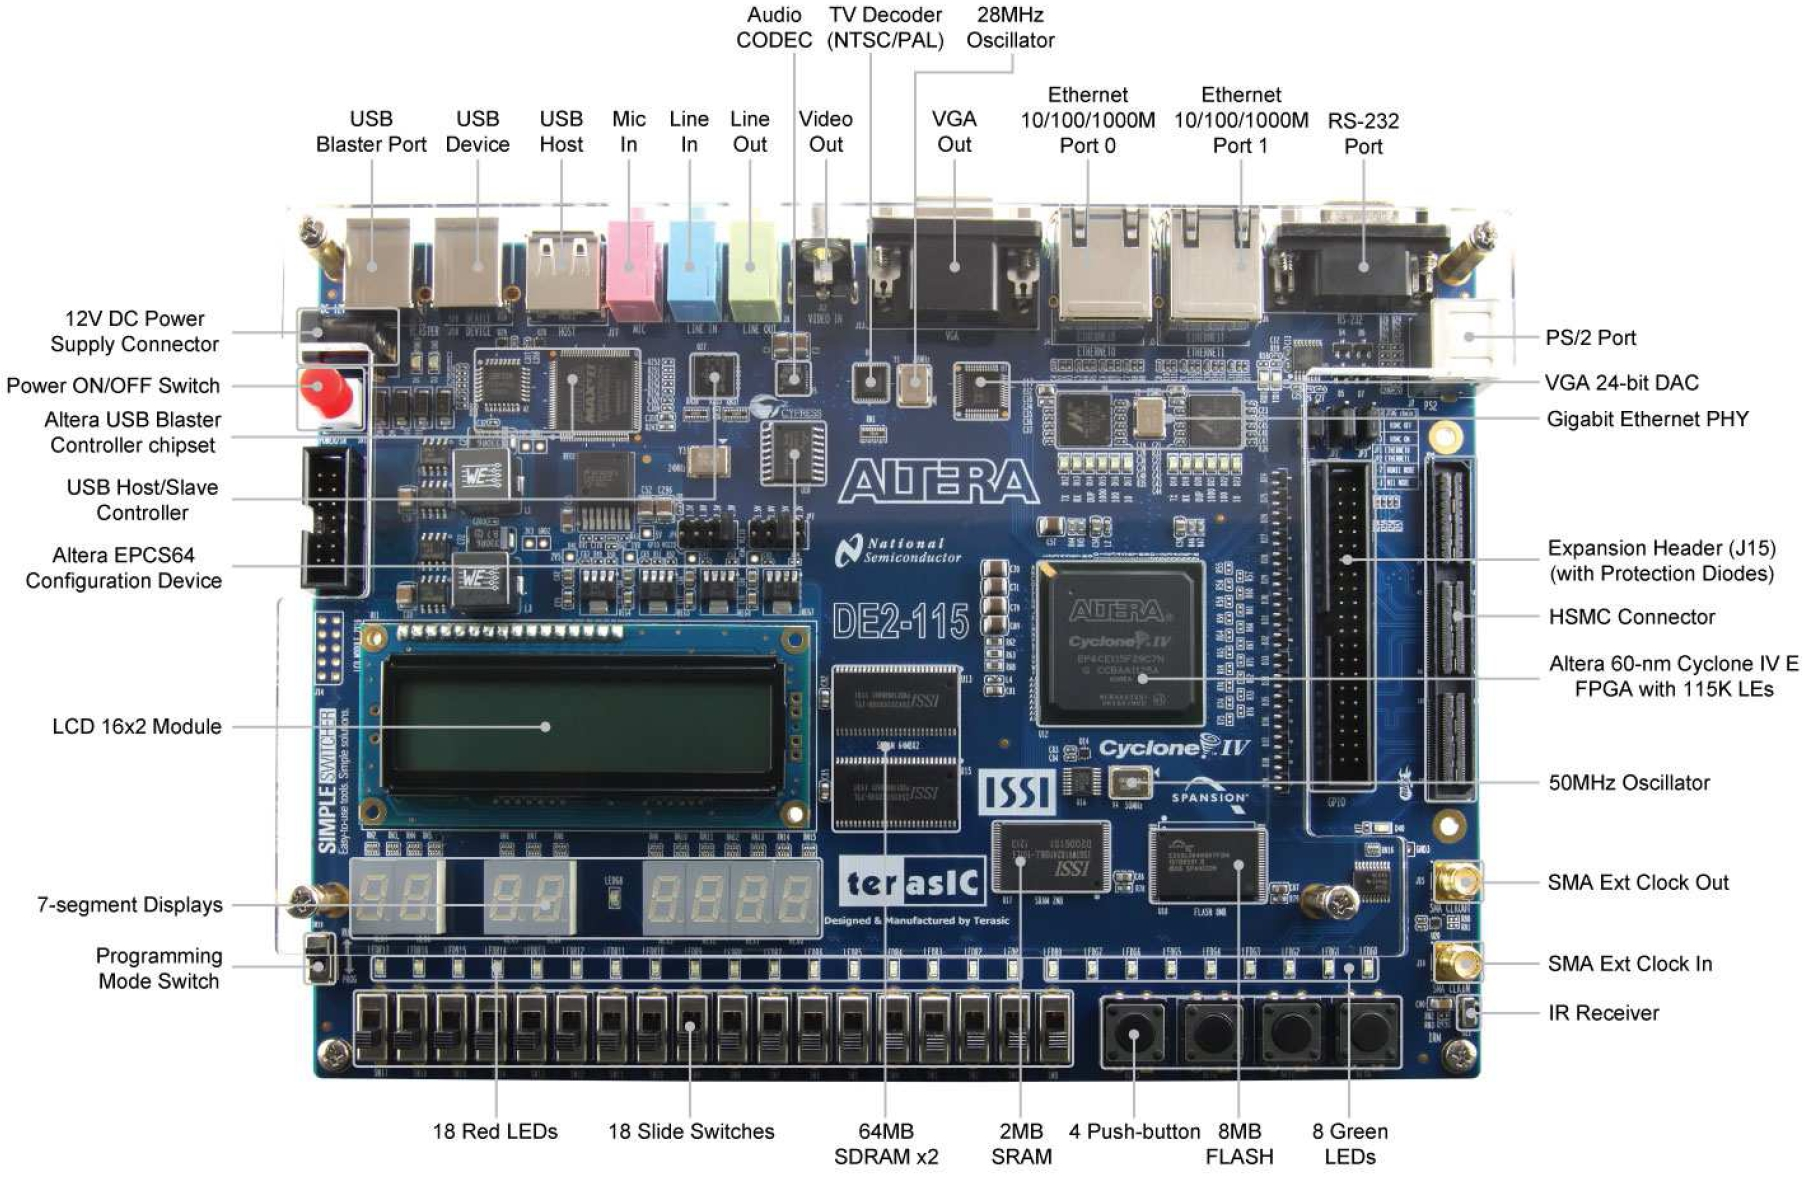
\includegraphics[width=0.93\textwidth]{img/fpga/terasic_placa_detalhado.jpg}
			\caption{FPGA de Desenvolvimento Altera DE2-115.}
			\label{fig:terasic_placa2}
		\end{figure}
	\end{frame}



\section{FPGA - Software}
	\begin{frame}{FPGA - Software - IDE de Desenvolvimento}
		\begin{figure}[p]
			\centering
			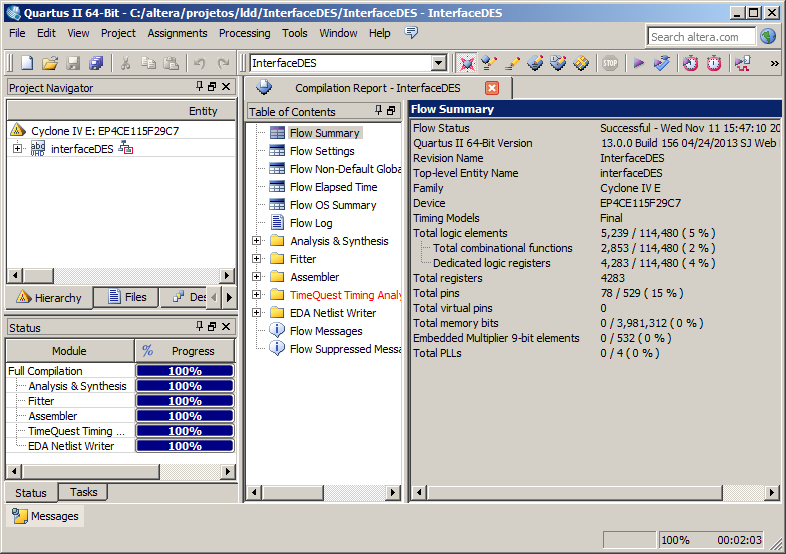
\includegraphics[width=0.7\textwidth]{img/fpga/altera.png}
			\caption{Altera Quartus II.}
			\label{fig:alteraquartus}
		\end{figure}
	\end{frame}
	
	\begin{frame}{FPGA - Software - IDE de Desenvolvimento - Desenvolvendo um Projeto}
		\begin{figure}[p]
			\centering
			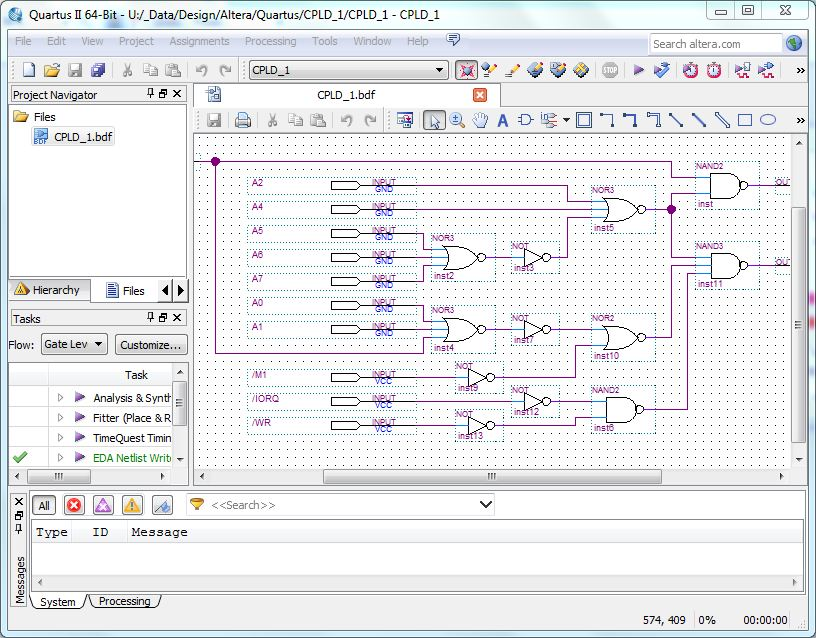
\includegraphics[width=0.63\textwidth]{img/fpga/software_quartus_portas.jpg}
			\caption{Projeto com assistência computacional usando portas lógicas.}
			\label{fig:alteraquartus_portas1}
		\end{figure}
	\end{frame}
	
	\begin{frame}{FPGA - Software - IDE de Desenvolvimento - Desenvolvendo um Projeto }
		\begin{figure}[p]
			\centering
			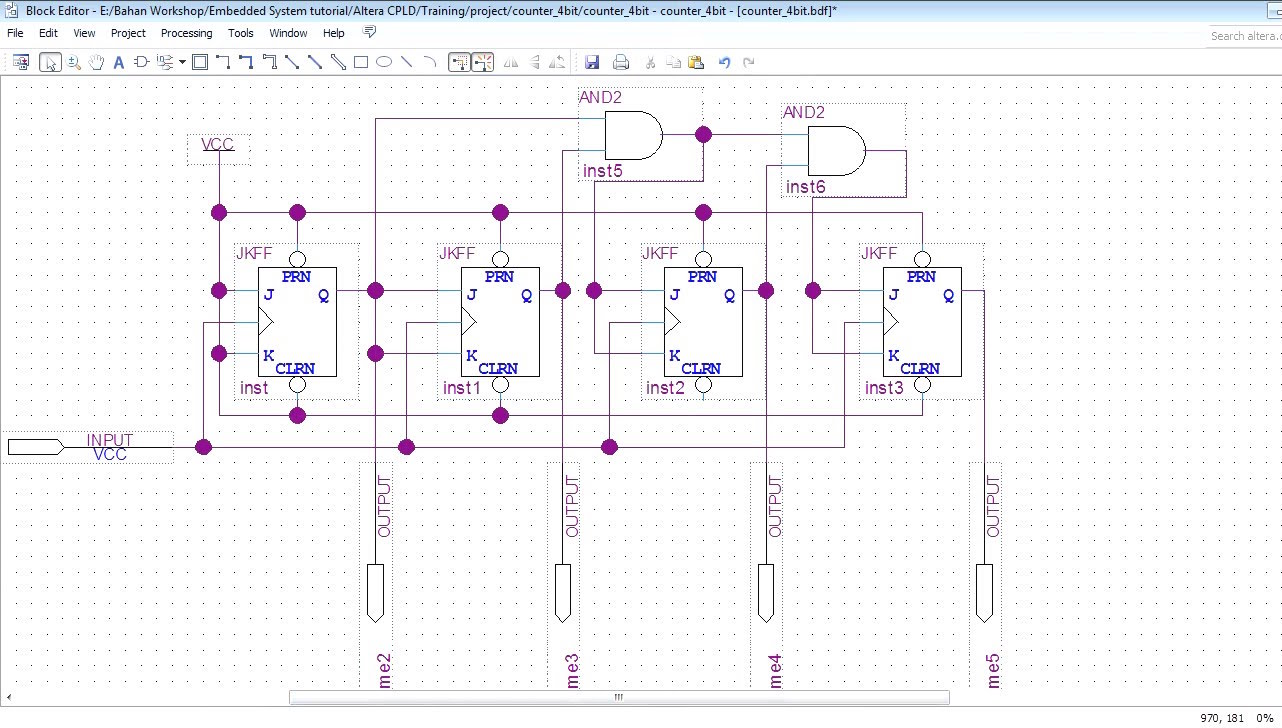
\includegraphics[width=0.85\textwidth]{img/fpga/software_quartus_portas2.jpg}
			\caption{Projeto Contador 4-bit usando portas lógicas.}
			\label{fig:alteraquartus_portas2}
		\end{figure}
	\end{frame}
	
	\begin{frame}{FPGA - Software - IDE de Desenvolvimento - Desenvolvendo um Projeto }
		\begin{figure}[p]
			\centering
			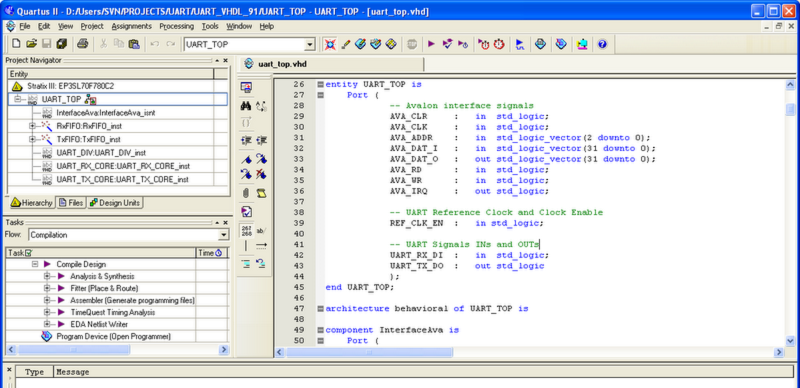
\includegraphics[width=1\textwidth]{img/fpga/software_quartus_vhdl.png}
			\caption{Projeto de uma interface UART usando VHDL.}
			\label{fig:alteraquartus_portas}
		\end{figure}
	\end{frame}
	
	\begin{frame}{FPGA - Software - IDE de Desenvolvimento - Desenvolvendo um Projeto }
		\begin{figure}[p]
			\centering
			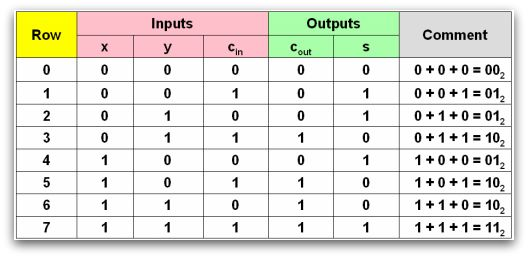
\includegraphics[width=1\textwidth]{img/fpga/adder-table.jpg}
			\caption{Somador Completo.}
			\label{fig:somador_completo}
		\end{figure}
	\end{frame}
	
	\begin{frame}{FPGA - Software - IDE de Desenvolvimento - Desenvolvendo um Projeto }
		\begin{figure}[p]
			\centering
			
\includegraphics[width=0.77\textwidth]{img/fpga/adder.png}
			\caption{Representação do Somador Completo em Portas Lógicas.}
			\label{fig:somador_completo_pl}
		\end{figure}
	\end{frame}
	
	\begin{frame}%{FPGA - Software - IDE de Desenvolvimento - Desenvolvendo um Projeto }
		\begin{figure}[p]
			\centering
			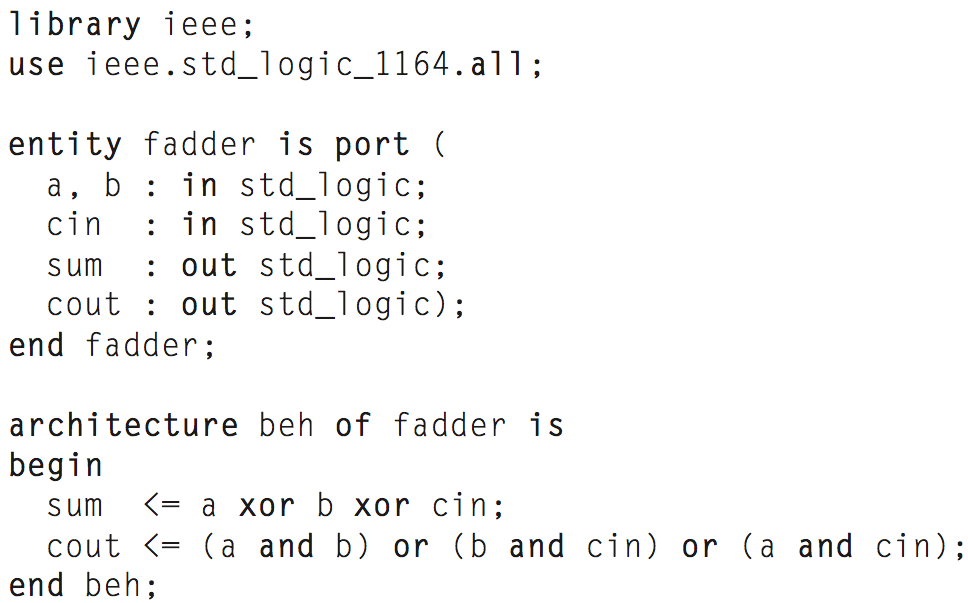
\includegraphics[width=0.9\textwidth]{img/fpga/code_vhdl.png}
			\caption{Código do Somador Completo em VHDL.}
			\label{fig:codigo_vhdl}
		\end{figure}
	\end{frame}
	
	
	\begin{frame}{FPGA - Software - IDE de Desenvolvimento - Desenvolvendo um Projeto}
		\begin{figure}[p]
			\centering
			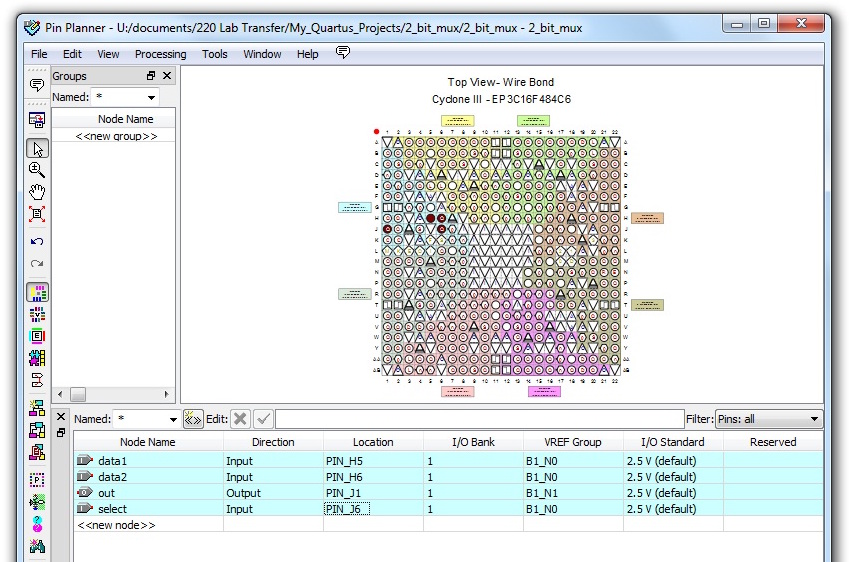
\includegraphics[width=0.74\textwidth]{img/fpga/software_quartus_pin.jpg}
			\caption{Pin Planner.}
			\label{fig:alteraquartus_pinagem}
		\end{figure}
	\end{frame}
	
	\begin{frame}%{FPGA - Software - IDE de Desenvolvimento - Desenvolvendo um Projeto}
		\begin{figure}[p]
			\centering
			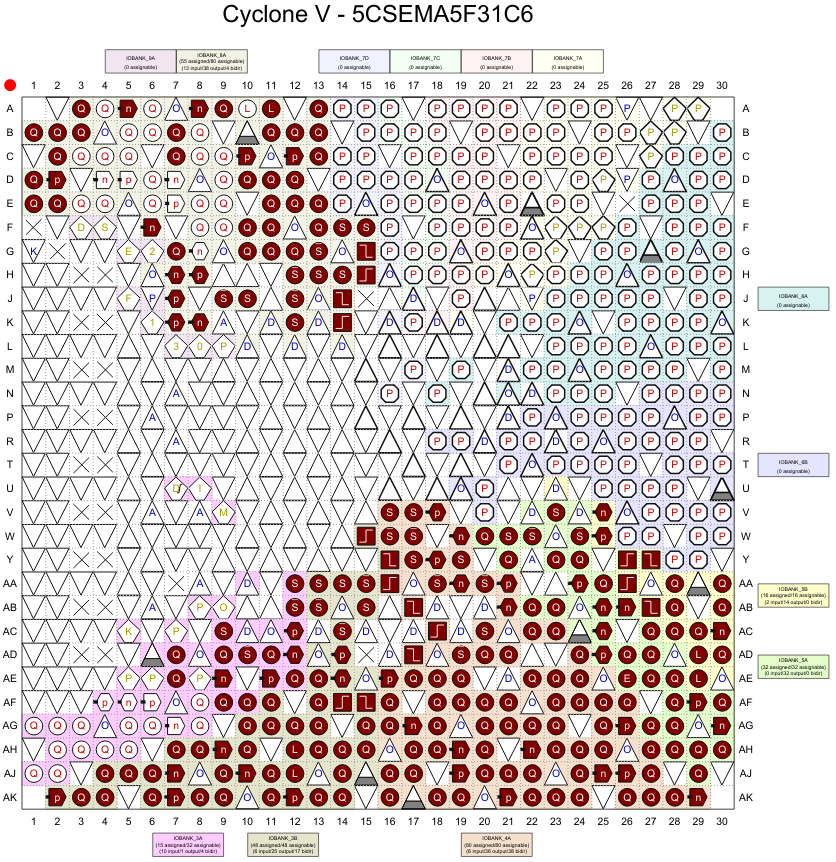
\includegraphics[width=0.6\textwidth]{img/fpga/pinplanner.png}
			\caption{Pin Planner aproximado.}
			\label{fig:pinplanner}
		\end{figure}
	\end{frame}
	
	\begin{frame}{FPGA - Software - IDE de Desenvolvimento - Compilando um Projeto}
		\begin{figure}[p]
			\centering
			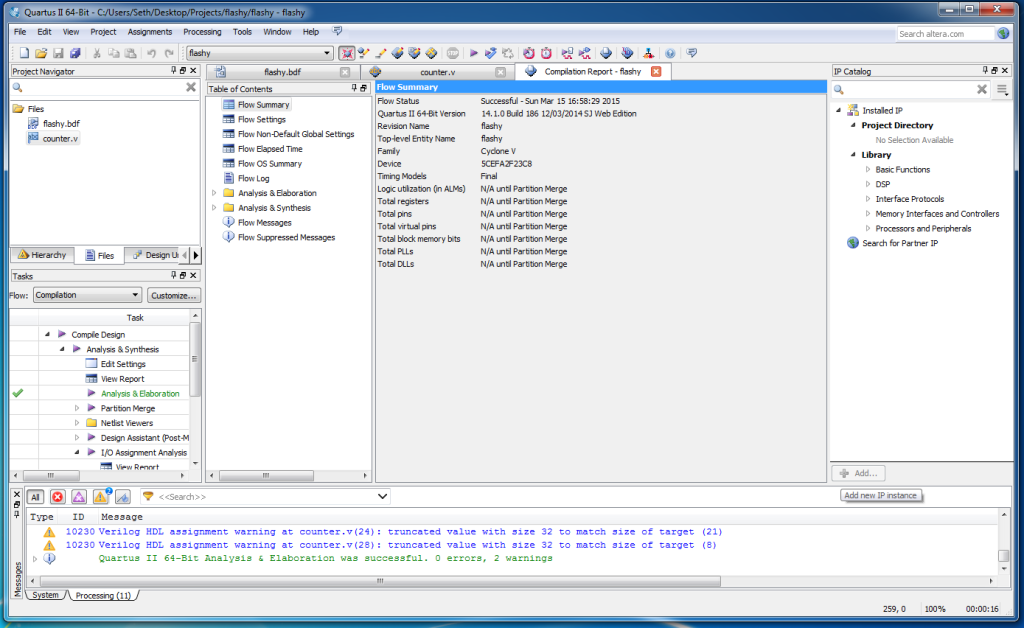
\includegraphics[width=0.8\textwidth]{img/fpga/software_quartus_compilation0.png}
			\caption{Início de síntese de um projeto.}
			\label{fig:alteraquartus_comp0}
		\end{figure}
	\end{frame}
	
	\begin{frame}{FPGA - Software - IDE de Desenvolvimento}
		\begin{figure}[p]
			\centering
			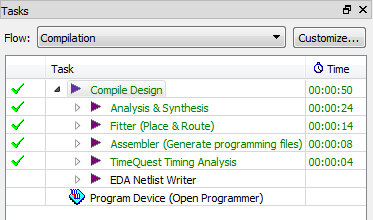
\includegraphics[width=0.8\textwidth]{img/fpga/software_quartus_compilation1.png}
			\caption{Término de síntese de um projeto.}
			\label{fig:alteraquartus_comp1}
		\end{figure}
	\end{frame}
	
	\begin{frame}{FPGA - Software - IDE de Desenvolvimento}
		\begin{figure}[p]
			\centering
			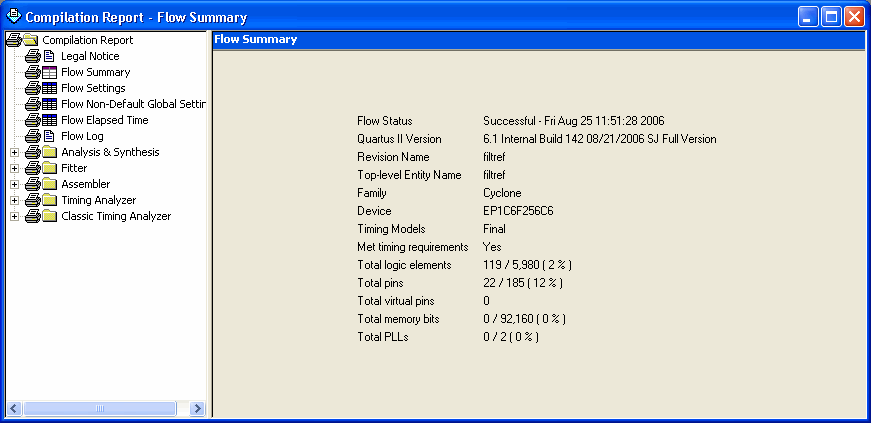
\includegraphics[width=1\textwidth]{img/fpga/software_quartus_compilation2.png}
			\caption{Relatório de compilação final.}
			\label{fig:alteraquartus_comp2}
		\end{figure}
	\end{frame}
	
	\begin{frame}{FPGA - Software - IDE de Desenvolvimento}
		\begin{figure}[p]
			\centering
			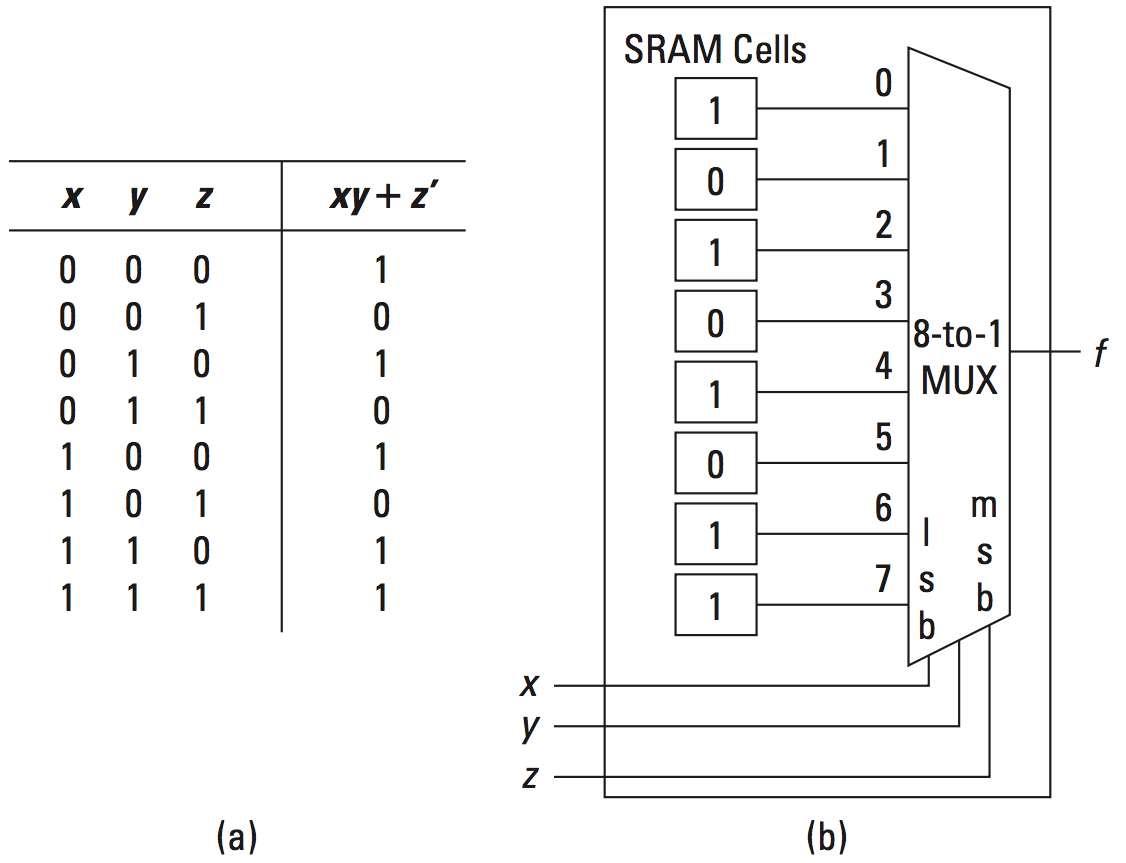
\includegraphics[width=0.6\textwidth]{img/fpga/funcao-geradora.png}
			\caption{Gerador de Função. a) tabela verdade e b) Look-Up Table (LUT) com Flip-flops para armazenamento.}
			\label{fig:funcao-geradora}
		\end{figure}
	\end{frame}
	
	
	
	
	\begin{frame}{FPGA - Software - IDE de Simulação}
		\begin{figure}[p]
			\centering
			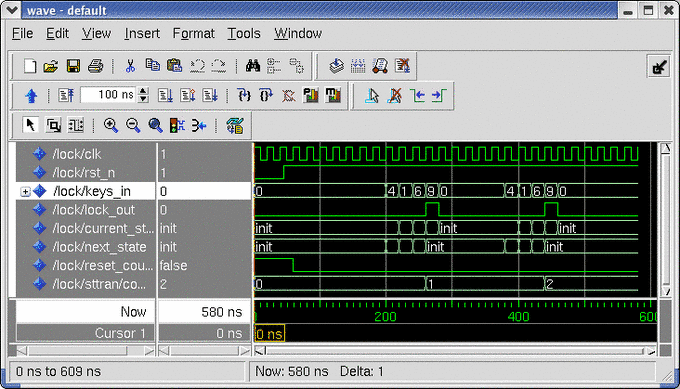
\includegraphics[width=0.85\textwidth]{img/fpga/modelsim.png}
			\caption{ModelSim.}
			\label{fig:modelsim}
		\end{figure}
	\end{frame}



\section{FPGA - Programação}
\begin{frame}{FPGA - Programação}
	\begin{itemize}
		\setlength\itemsep{1.0em}
		\item A implementação na placa FPGA é feita por:
		\begin{itemize}
			\setlength\itemsep{0.5em}
			\item Linguagens de descrição chamadas de \textbf{Linguagens de Descrição de \textit{Hardware} (HDL)}
			\begin{itemize}
				\item São algumas linguagens: VHDL \textit{(foto)}, Verilog, ABEL, etc..
			\end{itemize}
			
			\item Ou por meio do desenvolvimento de \textbf{diagramas esquemáticos com ferramentas gráficas assistidas pelo computador} \textit{(foto)}.
			
			\item Hoje, também é possível escrever por meio de \textbf{linguagens de alto nível} para como Handel-C, C-like ou mesmo o SystemC.
		\end{itemize}
		
		\item Alguns conceitos de fundamentais sobre linguagens de descrição de \textit{hardware}:
		\begin{itemize}
			\setlength\itemsep{0.5em}
			\item Estas linguagens permitem por exemplo \textit{loops} infinitos ou portas lógicas com inúmeras entradas;
			
			\item Essas são possível serem descritas em \textit{software} mas impossível de implementar em \textit{hardware}.
		\end{itemize}
	\end{itemize}
\end{frame}
	
	\begin{frame}{FPGA - Programação}
		\begin{figure}[p]
			\centering
			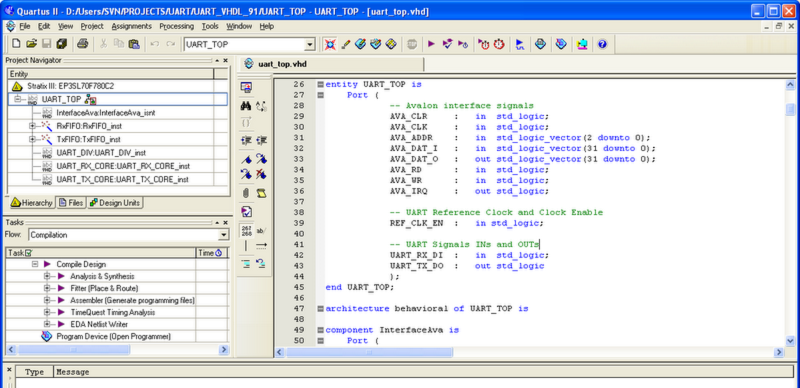
\includegraphics[width=1\textwidth]{img/fpga/software_quartus_vhdl.png}
			\caption{Projeto de uma interface UART usando VHDL.}
			\label{fig:alteraquartus_vhdl-2}
		\end{figure}
	\end{frame}
	
	\begin{frame}{FPGA - Programação}
		\begin{itemize}
			\setlength\itemsep{1.0em}
			\item A implementação na placa FPGA é feita por:
			\begin{itemize}
				\setlength\itemsep{0.5em}
				\item Linguagens de descrição chamadas de \textbf{Linguagens de Descrição de \textit{Hardware} (HDL)}
				\begin{itemize}
					\item São algumas linguagens: VHDL, Verilog, ABEL, etc..
				\end{itemize}
				
				\item Ou por meio do desenvolvimento de \textbf{diagramas esquemáticos com ferramentas gráficas assistidas pelo computador}.
				
				\item Hoje, também é possível escrever por meio de \textbf{linguagens de alto nível} para como Handel-C ou mesmo o SystemC.
			\end{itemize}
			
			\item Alguns conceitos de fundamentais sobre linguagens de descrição de \textit{hardware}:
			\begin{itemize}
				\setlength\itemsep{0.5em}
				\item Estas linguagens permitem por exemplo \textit{loops} infinitos ou portas lógicas com inúmeras entradas;
				
				\item Essas são possível serem descritas em \textit{software} mas impossível de implementar em \textit{hardware}.
			\end{itemize}
		\end{itemize}
	\end{frame}
	
	\begin{frame}{FPGA - Programação}
		\begin{figure}[p]
			\centering
			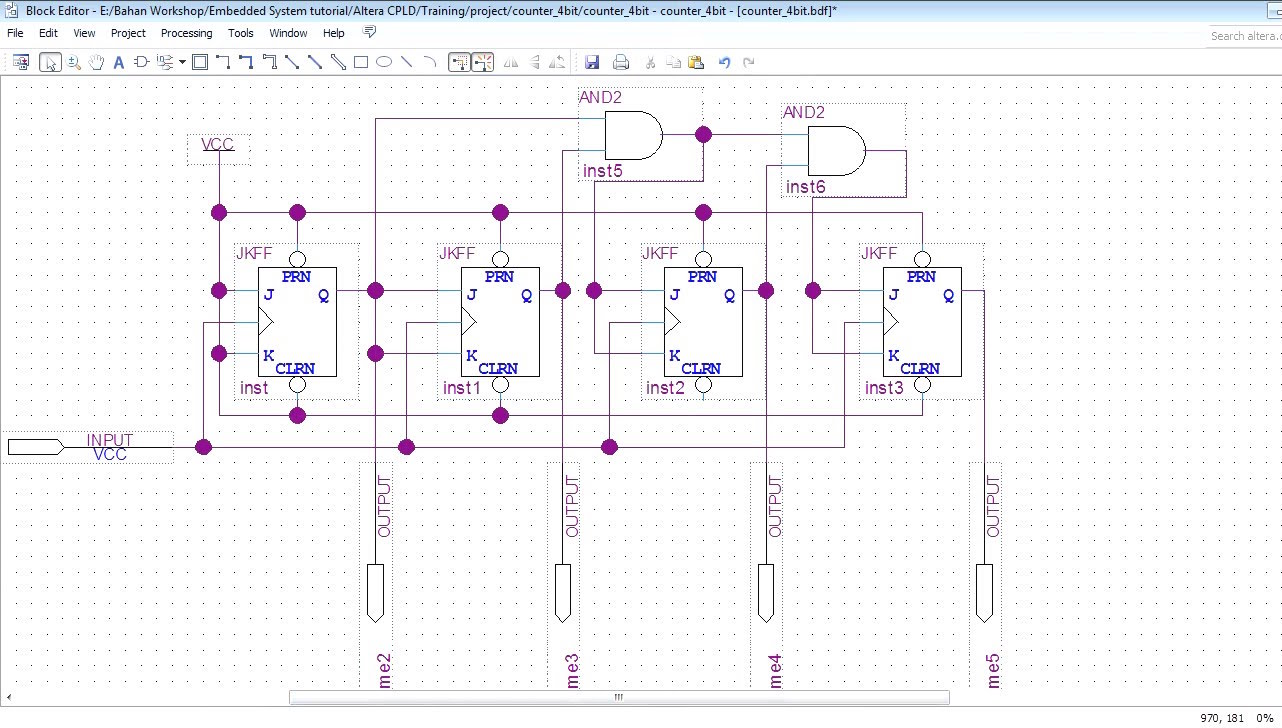
\includegraphics[width=0.85\textwidth]{img/fpga/software_quartus_portas2.jpg}
			\caption{Projeto Contador 4-bit usando portas lógicas.}
			\label{fig:alteraquartus_portas2-2}
		\end{figure}
	\end{frame}
	
	\begin{frame}{FPGA - Programação}
		\begin{itemize}
			\setlength\itemsep{1.0em}
			\item A implementação na placa FPGA é feita por:
			\begin{itemize}
				\setlength\itemsep{0.5em}
				\item Linguagens de descrição chamadas de \textbf{Linguagens de Descrição de \textit{Hardware} (HDL)}
				\begin{itemize}
					\item São algumas linguagens: VHDL, Verilog, ABEL, etc..
				\end{itemize}
				
				\item Ou por meio do desenvolvimento de \textbf{diagramas esquemáticos com ferramentas gráficas assistidas pelo computador}.
				
				\item Hoje, também é possível escrever por meio de \textbf{linguagens de alto nível} para como Handel-C ou mesmo o SystemC.
			\end{itemize}
			
			\item Alguns conceitos de fundamentais sobre linguagens de descrição de \textit{hardware}
			\begin{itemize}
				\setlength\itemsep{0.5em}
				\item Estas linguagens permitem por exemplo \textit{loops} infinitos ou portas lógicas com inúmeras entradas;
				
				\item Essas são possível serem descritas em \textit{software} mas impossível de implementar em \textit{hardware}.
			\end{itemize}
		\end{itemize}
	\end{frame}
	
	
	
	
	\begin{frame}{FPGA - Programação - VHDL}
		\begin{itemize}
			\setlength\itemsep{1.3em}
			\item Linguagem para descrever o \textbf{comportamento} e \textbf{estrutura} de um sistema digital.
			
			\item A abreviatura VHDL significa \textit{\underline{VHSIC Hardware Description Language}} 
			\begin{itemize}
				\item Sendo que VHSIC significa \textit{\underline{Very High Speed Integrated Circuit}}. 
			\end{itemize}
			
			\item Ou seja, seu nome em português é \textbf{Linguagem de Descrição de \textit{Hardware} de Circuitos Integrados com Altíssima Velocidade}. 
			
			\item Ela tem propriedades suficientes para ser \textbf{independente tecnologicamente}
			\begin{itemize}
				\item Ou seja, a mesma linguagem VHDL utilizada para descrever as tecnologias de hoje, poderá descrever as futuras tecnologias \cite{Roth1998}.
			\end{itemize}
		\end{itemize}
	\end{frame}
	
	
	\begin{frame}[fragile]{FPGA - Programação - VHDL}
		\begin{minted}[mathescape,linenos, numbersep=5pt, gobble=2, tabsize=3, frame=lines, framesep=2mm]{vhdl}
		C <= A and B; 
		E <= C or D;
		\end{minted}
		\pause
		\begin{figure}[h]
			\centering
			\caption{Altera Cyclone IV acoplado à placa da Terasic Altera DE2-115}
			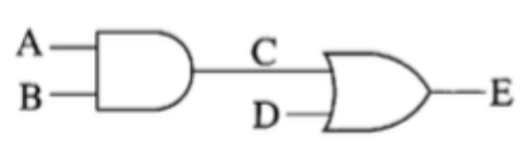
\includegraphics[height=0.2\textheight]{img/fpga/vhdl.png}
			\label{fig:vhdl}
		\end{figure}
\end{frame}

	\begin{frame}{FPGA - Bibliografia}
		\begin{multicols}{2}
			\begin{figure}[p]
				\centering
				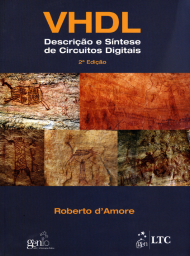
\includegraphics[width=0.33\textwidth]{img/fpga/l4.png}
				\caption{VHDL: Descrição e síntese de circuitos digitais \cite{DAmore2005}.}
				\label{fig:l4}
			\end{figure}
			\columnbreak
			\begin{figure}[p]
				\centering
				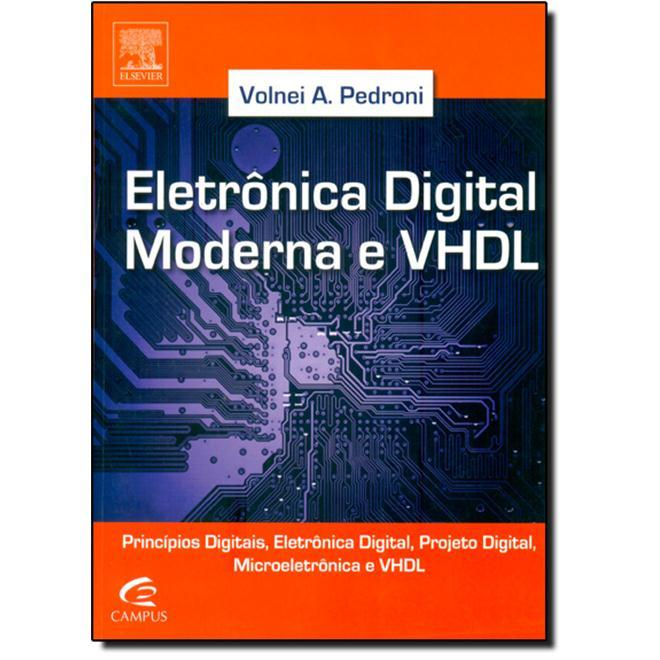
\includegraphics[width=0.45\textwidth]{img/fpga/l5.jpg}
				\caption{Eletrônica Digital Moderna e VHDL.  \cite{PEDRONI2010}.}
				\label{fig:l5}
			\end{figure}
		\end{multicols}
	\end{frame}
	
	
	\begin{frame}{FPGA - Bibliografia}
		\begin{figure}[p]
			\centering
			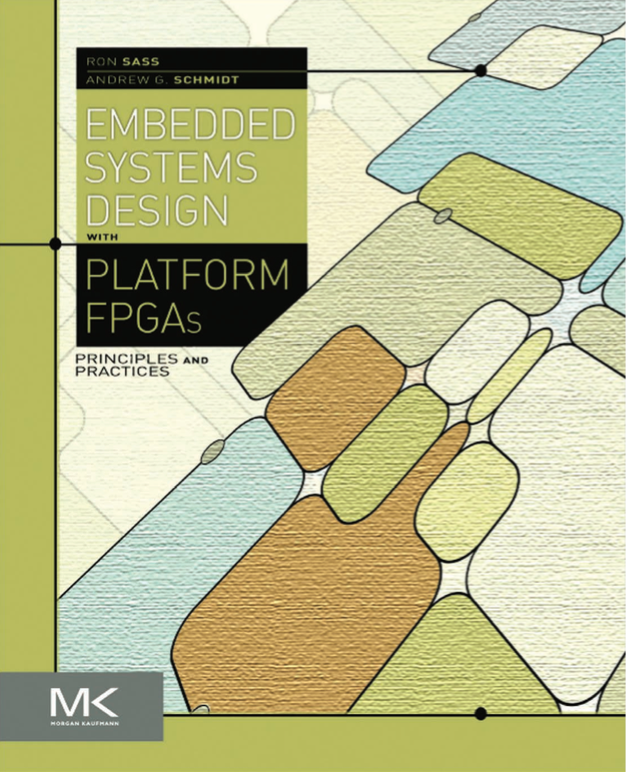
\includegraphics[width=0.38\textwidth]{img/fpga/l6.png}
			\caption{\textit{Embedded Systems Design with Platform FPGAs,
				Principles and Practices} \cite{Sass2010} .}
			\label{fig:l6}
		\end{figure}
	\end{frame}


	\begin{frame}{FPGA - Vantagens e Desvantagens}
		\begin{itemize}
			\item Vantagens:
			\begin{itemize}
				\setlength\itemsep{0.2em}
				\item Não é necessário uma ASIC pra realizar testes:
				\begin{itemize}
					\item Com o uso do FPGA, é possível fazer os testes necessários prevendo erros;
				\end{itemize}
				
				\item É possível adicionar mais recursos em sua placa para que o projeto tente simular o mais próximo possível do produto final
				\begin{itemize}
					\item Câmeras, telas \textit{touch} ...
				\end{itemize}
				
				\item Amplamente usado para didática para a construção de circuitos integrados;
				
				\item Aplicação em diversas áreas inclusive áreas de grande importância como projetos no qual necessita de sistema críticos
				\begin{itemize}
					\item A Nasa...
					\item A Intel... \textit{(foto)}
				\end{itemize}
			\end{itemize}
			
				\bigskip
			
			\item Desvantagens:
			\begin{itemize}
				\setlength\itemsep{0.2em}
				\item Seu custo é bastante elevado para a utilização em projetos pequenos;
				
				\item Ele não possui capacidade de usar recurso analógicos;
				
				\item Seu desempenho entra em desvantagem em comparação com placas ASIC.
			\end{itemize}
		\end{itemize}
	\end{frame}
	
	\begin{frame}
		\begin{figure}[H]
			\centering
			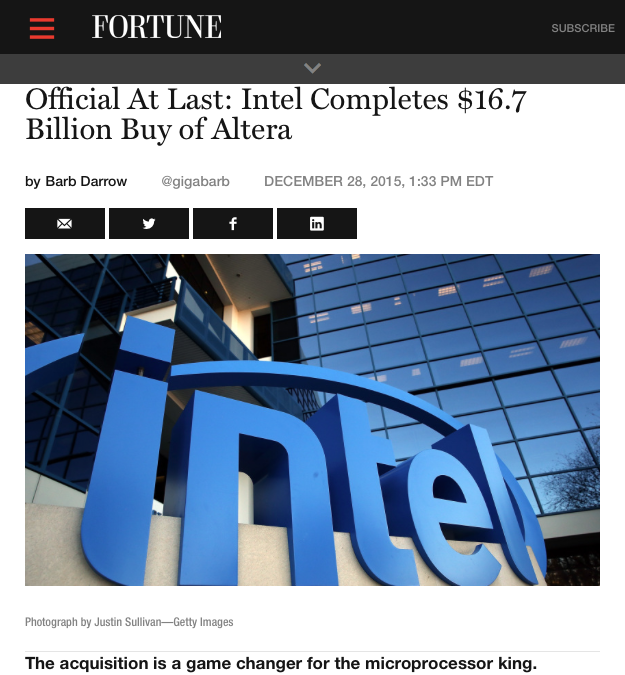
\includegraphics[width=0.5\textwidth]{img/fpga/intel_altera_2.png}
			\protect\caption{Noticiário. Fonte: \url{http://fortune.com/2015/12/28/intel-completes-altera-acquisition/}}
			\label{fig:intel_altera_noticia}
		\end{figure}
	\end{frame}
	
	\begin{frame}{FPGA - Vantagens e Desvantagens}
		\begin{itemize}
			\item Vantagens:
			\begin{itemize}
				\setlength\itemsep{0.2em}
				\item Não é necessário uma ASIC pra realizar testes:
				\begin{itemize}
					\item Com o uso do FPGA, é possível fazer os testes necessários prevendo erros;
				\end{itemize}
				
				\item É possível adicionar mais recursos em sua placa para que o projeto tente simular o mais próximo possível do produto final
				\begin{itemize}
					\item Câmeras, telas \textit{touch} ...
				\end{itemize}
				
				\item Amplamente usado para didática para a construção de circuitos integrados;
				
				\item Aplicação em diversas áreas inclusive áreas de grande importância como projetos no qual necessita de sistema críticos
				\begin{itemize}
					\item A Nasa...
					\item A Intel...
				\end{itemize}
			\end{itemize}
			
			\bigskip
			
			\item Desvantagens:
			\begin{itemize}
				\setlength\itemsep{0.2em}
				\item Seu custo é bastante elevado para a utilização em projetos pequenos;
				
				\item Ele não possui capacidade de usar recurso analógicos;
				
				\item Seu desempenho entra em desvantagem em comparação com placas ASIC.
			\end{itemize}
		\end{itemize}
	\end{frame}

\section{UFOP - Laboratório iMobilis}
	\begin{frame}{Kit Odyssey}
		\begin{multicols}{2}
				\begin{figure}[h]
					\centering
					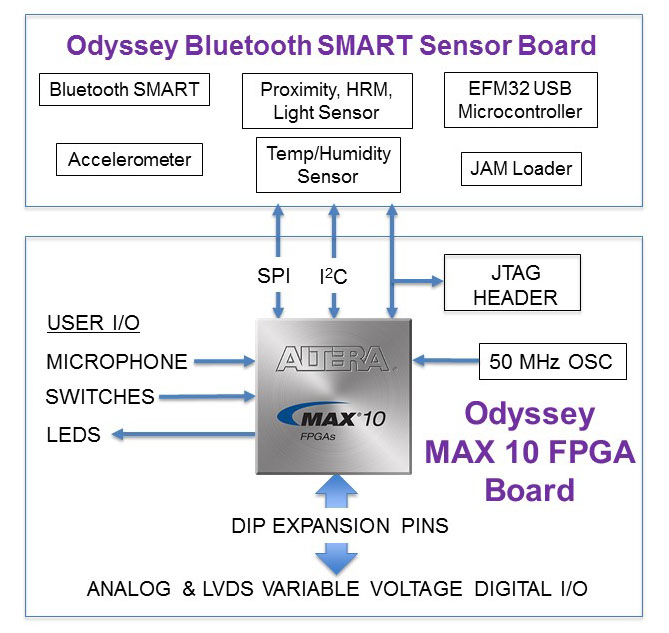
\includegraphics[width=0.49\textwidth]{img/imobilis/odyssey-esquematico.jpg}
					\caption{Esquemático do Odyssey IV.}
					\label{fig:odyssey-esquematico}
				\end{figure}
			\columnbreak
				\begin{itemize}
					\item Características:
					\begin{itemize}
						\setlength\itemsep{1em}
						\item Altera FPGA 10M08;
						\item 8 mil elementos lógicos
						\item 169 pinos;
						\item 55 nm.
					\end{itemize}
				\end{itemize}
		\end{multicols}
	\end{frame}
	
	\begin{frame}{Kit Odyssey}
		\begin{figure}[h]
			\centering
			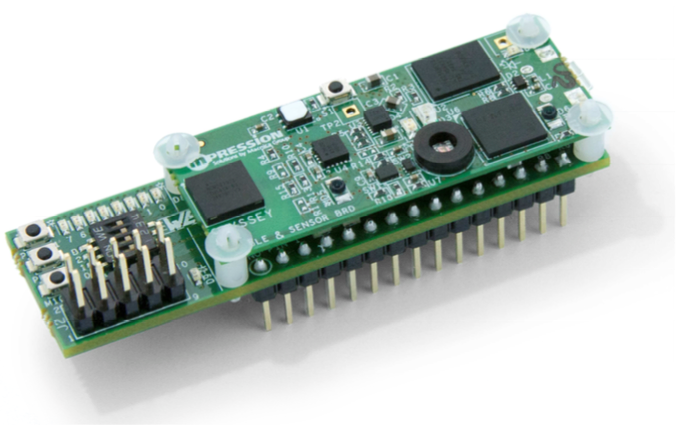
\includegraphics[width=0.7\textwidth]{img/imobilis/odyssey-foto.png}
			\caption{Odyssey IV.}
			\label{fig:odyssey-foto}
		\end{figure}
	\end{frame}
	
	
	\begin{frame}{Kit Mercurio IV}
		\begin{itemize}
			\item Modelo EP4CE30F23 responsável possui cerca de $ 30 $ mil elementos lógicos, com $ 484 $ pinos de entrada e saída e utiliza \textit{clock} de $50Mhz$.
		\end{itemize}
		
		\begin{figure}[h]
			\centering
			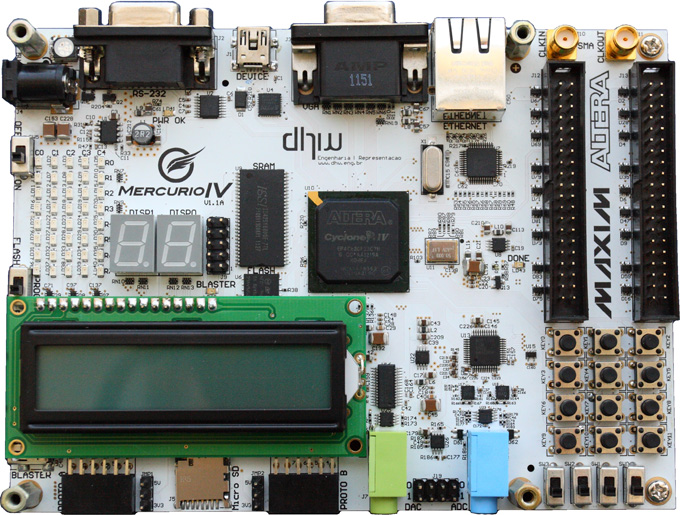
\includegraphics[width=0.55\textwidth]{img/imobilis/mercurio-foto.jpg}
			\caption{Mercurio IV.}
			\label{fig:mercurio-foto}
		\end{figure}
	\end{frame}
	
	\begin{frame}%{Kit Mercurio IV}
		\begin{figure}[h]
			\centering
			\includegraphics[width=0.73\textwidth]{img/imobilis/mercurio-esquematico.png}
			\caption{Pespectiva Geral dos Componentes do Mercurio IV.}
			\label{fig:mercurio-esquematico}
		\end{figure}
	\end{frame}
	
	
	\begin{frame}{Kit Helio Cyclone V}
		\begin{itemize}
			\setlength\itemsep{1em}
			\item Fabricado em tecnologia de silício de 28nm.
			
			\item Este FPGA integra num único dispositivo um sistema em \textit{hardware} baseado no processador ARM Cortex A9 dual-core e mais um grande conjunto de periféricos.
			
			\item Características:
			\begin{itemize}
				\setlength\itemsep{0.4em}
				\item Altera Cyclone V SoC -- 5CSXFC6C6U23C8NES / 5CSXFC5C6U23C7N
				\item HSMC expansion connector
				\item DDR3-SDRAM
				\item Micro SD Card
				\item Interfaces: 1Gb Ethernet, USB OTG, UART...
				\item Yocto Linux BSP
			\end{itemize}
		\end{itemize}
	\end{frame}
	
	\begin{frame}{Kit Helio Cyclone V}
		\begin{figure}[h]
			\centering
			\includegraphics[width=0.8\textwidth]{img/imobilis/helio-foto.jpg}
			\caption{Componentes do Helio Cyclone V.}
			\label{fig:helio-foto}
		\end{figure}
	\end{frame}
	
	\begin{frame}%{Kit Helio Cyclone V}
		\begin{figure}[h]
			\centering
			\includegraphics[width=1\textwidth]{img/imobilis/helio-foto-2.png}
			\caption{Componentes do Helio Cyclone V.}
			\label{fig:helio-foto2}
		\end{figure}
	\end{frame}
	
	\begin{frame}%{Kit Helio Cyclone V}
		\begin{figure}[h]
			\centering
			\includegraphics[width=0.59\textwidth]{img/imobilis/helio-esquematico.png}
			\caption{Esquemático do Helio Cyclone V.}
			\label{fig:helio-esquematico}
		\end{figure}
	\end{frame}
	
	
\maketitle

\section{Bibliografia}

\bibliographystyle{abbrv}
\bibliography{sbc-template}

\maketitle

\end{document}
